\section{Übung 3 – Zufallssignale}

In dieser Übung werden empirische Kenngrößen (Lage- und Streumaße) sowie die
empirische Korrelation zeitdiskreter Zufallssignale bestimmt. Alle Signalwerte
sind den Stem-Plots bzw.\ dem Histogramm des Aufgabenblattes entnommen. Es
gelten durchgängig die Definitionen aus Abschnitt~\ref{sec:kenngroessen-zufaellige-signale}
(empirischer Mittelwert und Median: Abschnitt~\ref{sec:lagemasse}; empirische
Varianz und Standardabweichung: Abschnitt~\ref{sec:streumasse}; empirische
Kreuzkorrelation: Abschnitt~\ref{sec:empirische-korrelation}).

% ================================================================
\subsection*{Vorrechenaufgabe 3 – Statistische Kenngrößen von Signalen}
% ================================================================

Aus dem Stem-Plot liest man für $k = 0, \ldots, 16$ (also $N = 17$ Abtastwerte)
die folgenden Amplituden ab:

\begin{center}
\renewcommand{\arraystretch}{1.2}
\begin{tabular}{c|ccccccccccccccccc}
$k$    & 0 & 1 & 2 & 3 & 4 & 5 & 6 & 7 & 8 & 9 & 10 & 11 & 12 & 13 & 14 & 15 & 16 \\
\hline
$x[k]$ & $-1$ & $1$ & $0$ & $2$ & $\tfrac12$ & $-1$ & $2$ & $1$ & $1$ & $2$
       & $0$ & $-2$ & $1$ & $2$ & $1$ & $-1$ & $\tfrac12$ \\
\end{tabular}
\end{center}

\begin{center}
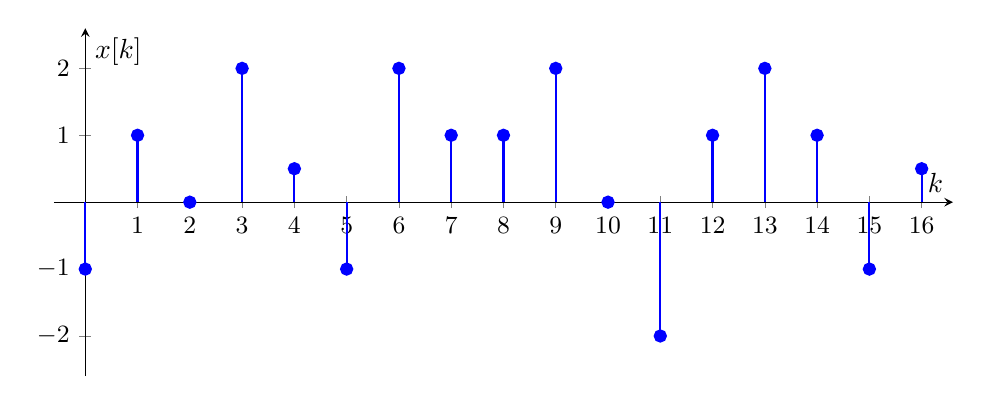
\begin{tikzpicture}
\begin{axis}[
  width=13cm, height=6cm,
  xmin=-0.6, xmax=16.6, ymin=-2.6, ymax=2.6,
  axis lines=middle,
  xlabel={$k$}, ylabel={$x[k]$},
  xtick={0,1,2,3,4,5,6,7,8,9,10,11,12,13,14,15,16},
  ytick={-2,-1,1,2},
  tick label style={font=\small},
  ymajorgrids=false,
]
\addplot+[ycomb, blue, thick, mark=*, mark options={blue}] coordinates {
  (0,-1) (1,1) (2,0) (3,2) (4,0.5) (5,-1) (6,2) (7,1) (8,1) (9,2)
  (10,0) (11,-2) (12,1) (13,2) (14,1) (15,-1) (16,0.5)
};
\end{axis}
\end{tikzpicture}
\end{center}

% ---- a) --------------------------------------------------------
\subsubsection*{a) Histogramm der Amplituden}

\begin{beispiel}[Histogramm der Signalamplituden]

\textbf{Gegeben:} Die $N = 17$ Amplitudenwerte des Signals $x[k]$.

\textbf{Gesucht:} Das Histogramm $f[x]$ (absolute Häufigkeit der auftretenden
Amplitudenwerte).

\textbf{Formel} (Histogramm als absolute Häufigkeit der Klassen,
Abschnitt~\ref{sec:kenngroessen-zufaellige-signale}):

$$
f[x] = \#\{\, k : x[k] = x \,\}
$$

\textbf{Rechnung:} Auszählen der auftretenden Amplitudenwerte:

\begin{center}
\renewcommand{\arraystretch}{1.2}
\begin{tabular}{c|cccccc|c}
$x$    & $-2$ & $-1$ & $0$ & $\tfrac12$ & $1$ & $2$ & $\sum$ \\
\hline
$f[x]$ & $1$  & $3$  & $2$ & $2$        & $5$ & $4$ & $17$ \\
\end{tabular}
\end{center}

Probe: $1 + 3 + 2 + 2 + 5 + 4 = 17 = N$. \checkmark

\begin{center}
\begin{tikzpicture}
\begin{axis}[
  width=11cm, height=6cm,
  ybar, bar width=18pt,
  xmin=-2.8, xmax=2.8, ymin=0, ymax=6,
  axis lines=left,
  xlabel={$x$}, ylabel={$f[x]$ (Häufigkeit)},
  xtick={-2,-1,0,0.5,1,2},
  xticklabels={$-2$,$-1$,$0$,$\tfrac12$,$1$,$2$},
  ytick={0,1,2,3,4,5},
  tick label style={font=\small},
  nodes near coords, nodes near coords style={font=\footnotesize},
]
\addplot[fill=blue!30, draw=blue!70] coordinates {
  (-2,1) (-1,3) (0,2) (0.5,2) (1,5) (2,4)
};
\end{axis}
\end{tikzpicture}
\end{center}

\textbf{Lösung:} Die Verteilung ist leicht linkslastig (Häufung bei $x = 1$ und
$x = 2$), mit einzelnen kleinen Ausreißern bei $x = -2$.

\end{beispiel}

% ---- b) --------------------------------------------------------
\subsubsection*{b) Empirischer Mittelwert}

\begin{beispiel}[Empirischer Mittelwert]

\textbf{Gegeben:} $N = 17$ Amplitudenwerte $x[k]$.

\textbf{Gesucht:} Der empirische Mittelwert $\hat{\bar{x}}$.

\textbf{Formel} (empirischer Mittelwert, Abschnitt~\ref{sec:lagemasse}):

$$
\hat{\bar{x}} = \frac{1}{N} \sum_{k=0}^{N-1} x[k]
$$

\textbf{Rechnung:} Am bequemsten über die Histogramm-Häufigkeiten:

$$
\sum_{k=0}^{16} x[k]
= (-2)\cdot 1 + (-1)\cdot 3 + 0\cdot 2 + \tfrac12\cdot 2 + 1\cdot 5 + 2\cdot 4
= -2 - 3 + 0 + 1 + 5 + 8 = 9
$$

$$
\hat{\bar{x}} = \frac{9}{17}
$$

\textbf{Lösung:}

$$
\boxed{\;\hat{\bar{x}} = \frac{9}{17} \approx 0{,}529\;}
$$

\end{beispiel}

% ---- c) --------------------------------------------------------
\subsubsection*{c) Median}

\begin{beispiel}[Median]

\textbf{Gegeben:} $N = 17$ Amplitudenwerte $x[k]$.

\textbf{Gesucht:} Der Median $\tilde{x}$.

\textbf{Formel} (Median als Mitte der geordneten Daten,
Abschnitt~\ref{sec:lagemasse}): Bei ungeradem $N$ ist

$$
\tilde{x} = x_{\left(\frac{N+1}{2}\right)}^{\text{sort}}
$$

das mittlere Element der aufsteigend sortierten Wertefolge.

\textbf{Rechnung:} Sortieren der $17$ Werte:

$$
-2,\; -1,\, -1,\, -1,\; 0,\, 0,\; \tfrac12,\, \tfrac12,\;
\underbrace{1}_{9.\ \text{Wert}},\, 1,\, 1,\, 1,\, 1,\; 2,\, 2,\, 2,\, 2
$$

Bei $N = 17$ ist der $\tfrac{N+1}{2} = 9$-te Wert der Median.

\textbf{Lösung:}

$$
\boxed{\;\tilde{x} = 1\;}
$$

\end{beispiel}

% ---- d) --------------------------------------------------------
\subsubsection*{d) Empirische Varianz}

\begin{beispiel}[Empirische Varianz]

\textbf{Gegeben:} $N = 17$, $\hat{\bar{x}} = \tfrac{9}{17}$.

\textbf{Gesucht:} Die empirische Varianz $\hat{\sigma}^2$.

\textbf{Formel} (empirische Varianz, Abschnitt~\ref{sec:streumasse}):

$$
\hat{\sigma}^2 = \frac{1}{N-1} \sum_{k=0}^{N-1} \bigl(x[k] - \hat{\bar{x}}\bigr)^2
= \frac{1}{N-1}\left( \sum_{k=0}^{N-1} x[k]^2 - N\,\hat{\bar{x}}^{\,2} \right)
$$

\textbf{Rechnung:} Zunächst die Summe der Quadrate (über die Häufigkeiten):

$$
\sum_{k=0}^{16} x[k]^2
= (-2)^2\cdot 1 + (-1)^2\cdot 3 + 0^2\cdot 2 + \left(\tfrac12\right)^2\cdot 2
  + 1^2\cdot 5 + 2^2\cdot 4
= 4 + 3 + 0 + \tfrac12 + 5 + 16 = 28{,}5
$$

$$
\hat{\sigma}^2 = \frac{1}{16}\left( 28{,}5 - 17\cdot\left(\frac{9}{17}\right)^2 \right)
= \frac{1}{16}\left( 28{,}5 - \frac{81}{17} \right)
= \frac{1}{16}\cdot \frac{807}{34}
= \frac{807}{544}
$$

\textbf{Lösung:}

$$
\boxed{\;\hat{\sigma}^2 = \frac{807}{544} \approx 1{,}483\;}
$$

\end{beispiel}

% ---- e) --------------------------------------------------------
\subsubsection*{e) Empirische Standardabweichung}

\begin{beispiel}[Empirische Standardabweichung]

\textbf{Gegeben:} $\hat{\sigma}^2 = \tfrac{807}{544} \approx 1{,}483$.

\textbf{Gesucht:} Die empirische Standardabweichung $\hat{\sigma}$.

\textbf{Formel} (Abschnitt~\ref{sec:streumasse}):

$$
\hat{\sigma} = \sqrt{\hat{\sigma}^2}
$$

\textbf{Rechnung:}

$$
\hat{\sigma} = \sqrt{\frac{807}{544}} = \sqrt{1{,}483\ldots}
$$

\textbf{Lösung:}

$$
\boxed{\;\hat{\sigma} \approx 1{,}218\;}
$$

\end{beispiel}

% ================================================================
\subsection*{Aufgabe 3.1 – Statistische Kenngrößen von Signalen}
% ================================================================

Für $k = 0, \ldots, 15$ (also $N = 16$ Abtastwerte) liest man aus dem Stem-Plot ab:

\begin{center}
\renewcommand{\arraystretch}{1.2}
\begin{tabular}{c|cccccccccccccccc}
$k$    & 0 & 1 & 2 & 3 & 4 & 5 & 6 & 7 & 8 & 9 & 10 & 11 & 12 & 13 & 14 & 15 \\
\hline
$x[k]$ & $0$ & $1$ & $0$ & $0$ & $1$ & $1$ & $5$ & $1$ & $0$ & $1$
       & $1$ & $7$ & $0$ & $0$ & $0$ & $1$ \\
\end{tabular}
\end{center}

\begin{center}
\begin{tikzpicture}
\begin{axis}[
  width=13cm, height=6cm,
  xmin=-0.6, xmax=15.6, ymin=0, ymax=7.6,
  axis lines=middle,
  xlabel={$k$}, ylabel={$x[k]$},
  xtick={0,1,2,3,4,5,6,7,8,9,10,11,12,13,14,15},
  ytick={1,2,3,4,5,6,7},
  tick label style={font=\small},
]
\addplot+[ycomb, blue, thick, mark=*, mark options={blue}] coordinates {
  (0,0) (1,1) (2,0) (3,0) (4,1) (5,1) (6,5) (7,1) (8,0) (9,1)
  (10,1) (11,7) (12,0) (13,0) (14,0) (15,1)
};
\end{axis}
\end{tikzpicture}
\end{center}

Häufigkeiten: der Wert $0$ tritt $7$-mal, der Wert $1$ tritt $7$-mal, der Wert $5$
einmal und der Wert $7$ einmal auf ($7+7+1+1 = 16$).

% ---- a) --------------------------------------------------------
\subsubsection*{a) Empirischer Mittelwert}

\begin{beispiel}[Empirischer Mittelwert]

\textbf{Gegeben:} $N = 16$ Amplitudenwerte $x[k]$.

\textbf{Gesucht:} $\hat{\bar{x}}$.

\textbf{Formel} (Abschnitt~\ref{sec:lagemasse}):

$$
\hat{\bar{x}} = \frac{1}{N} \sum_{k=0}^{N-1} x[k]
$$

\textbf{Rechnung:}

$$
\sum_{k=0}^{15} x[k] = 7\cdot 1 + 1\cdot 5 + 1\cdot 7 = 7 + 5 + 7 = 19,
\qquad
\hat{\bar{x}} = \frac{19}{16}
$$

\textbf{Lösung:}

$$
\boxed{\;\hat{\bar{x}} = \frac{19}{16} = 1{,}1875\;}
$$

\end{beispiel}

% ---- b) --------------------------------------------------------
\subsubsection*{b) Median}

\begin{beispiel}[Median]

\textbf{Gegeben:} $N = 16$ Amplitudenwerte $x[k]$.

\textbf{Gesucht:} $\tilde{x}$.

\textbf{Formel} (Abschnitt~\ref{sec:lagemasse}): Bei geradem $N$ ist der Median das
arithmetische Mittel der beiden mittleren Werte:

$$
\tilde{x} = \frac{1}{2}\left( x_{\left(\frac{N}{2}\right)}^{\text{sort}}
                              + x_{\left(\frac{N}{2}+1\right)}^{\text{sort}} \right)
$$

\textbf{Rechnung:} Sortieren der $16$ Werte:

$$
0,0,0,0,0,0,0,\; \underbrace{1}_{8.},\, \underbrace{1}_{9.},\, 1,1,1,1,1,\; 5,\, 7
$$

Der $8.$ und $9.$ Wert sind beide $1$:

$$
\tilde{x} = \frac{1 + 1}{2} = 1
$$

\textbf{Lösung:}

$$
\boxed{\;\tilde{x} = 1\;}
$$

\end{beispiel}

% ---- c) --------------------------------------------------------
\subsubsection*{c) Empirische Varianz}

\begin{beispiel}[Empirische Varianz]

\textbf{Gegeben:} $N = 16$, $\hat{\bar{x}} = \tfrac{19}{16}$.

\textbf{Gesucht:} $\hat{\sigma}^2$.

\textbf{Formel} (Abschnitt~\ref{sec:streumasse}):

$$
\hat{\sigma}^2 = \frac{1}{N-1}\left( \sum_{k=0}^{N-1} x[k]^2 - N\,\hat{\bar{x}}^{\,2} \right)
$$

\textbf{Rechnung:}

$$
\sum_{k=0}^{15} x[k]^2 = 7\cdot 1^2 + 1\cdot 5^2 + 1\cdot 7^2 = 7 + 25 + 49 = 81
$$

$$
\hat{\sigma}^2 = \frac{1}{15}\left( 81 - 16\cdot\left(\frac{19}{16}\right)^2 \right)
= \frac{1}{15}\left( 81 - \frac{361}{16} \right)
= \frac{1}{15}\cdot \frac{935}{16}
= \frac{935}{240}
$$

\textbf{Lösung:}

$$
\boxed{\;\hat{\sigma}^2 = \frac{935}{240} \approx 3{,}896\;}
$$

\end{beispiel}

% ---- d) --------------------------------------------------------
\subsubsection*{d) Empirische Standardabweichung}

\begin{beispiel}[Empirische Standardabweichung]

\textbf{Gegeben:} $\hat{\sigma}^2 = \tfrac{935}{240} \approx 3{,}896$.

\textbf{Gesucht:} $\hat{\sigma}$.

\textbf{Formel} (Abschnitt~\ref{sec:streumasse}):

$$
\hat{\sigma} = \sqrt{\hat{\sigma}^2}
$$

\textbf{Rechnung:}

$$
\hat{\sigma} = \sqrt{\frac{935}{240}} = \sqrt{3{,}896\ldots}
$$

\textbf{Lösung:}

$$
\boxed{\;\hat{\sigma} \approx 1{,}974\;}
$$

\end{beispiel}

% ---- e) --------------------------------------------------------
\subsubsection*{e) Mittlere absolute Abweichung vom Median}

\begin{beispiel}[Mittlere absolute Abweichung $\tilde{\Delta}$]

\textbf{Gegeben:} $N = 16$, Median $\tilde{x} = 1$.

\textbf{Gesucht:} Die mittlere absolute Abweichung

$$
\tilde{\Delta} = \frac{1}{N} \sum_{k=0}^{N-1} \bigl| x[k] - \tilde{x} \bigr|.
$$

\textbf{Formel:} wie in der Aufgabenstellung angegeben (Streumaß relativ zum
Median, vgl.\ Abschnitt~\ref{sec:streumasse}).

\textbf{Rechnung:} Die Beträge $|x[k] - 1|$ nach Häufigkeiten:

$$
\sum_{k=0}^{15} |x[k] - 1|
= 7\cdot|0-1| + 7\cdot|1-1| + 1\cdot|5-1| + 1\cdot|7-1|
= 7\cdot 1 + 0 + 4 + 6 = 17
$$

$$
\tilde{\Delta} = \frac{17}{16}
$$

\textbf{Lösung:}

$$
\boxed{\;\tilde{\Delta} = \frac{17}{16} = 1{,}0625\;}
$$

\end{beispiel}

% ================================================================
\subsection*{Aufgabe 3.2 – Histogramm}
% ================================================================

Gegeben ist das Histogramm der Signalamplituden mit den absoluten Häufigkeiten
$f[x]$ für die Amplitudenwerte $x = -3, \ldots, 3$:

\begin{center}
\renewcommand{\arraystretch}{1.2}
\begin{tabular}{c|ccccccc|c}
$x$    & $-3$ & $-2$ & $-1$ & $0$ & $1$ & $2$ & $3$ & $\sum$ \\
\hline
$f[x]$ & $1$  & $5$  & $13$ & $14$ & $9$ & $7$ & $1$ & $50$ \\
\end{tabular}
\end{center}

\begin{center}
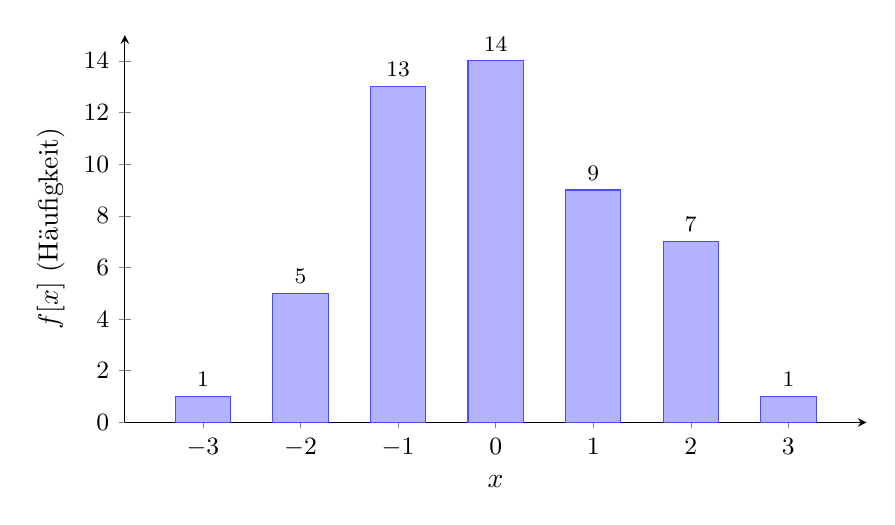
\begin{tikzpicture}
\begin{axis}[
  width=11cm, height=6.5cm,
  ybar, bar width=20pt,
  xmin=-3.8, xmax=3.8, ymin=0, ymax=15,
  axis lines=left,
  xlabel={$x$}, ylabel={$f[x]$ (Häufigkeit)},
  xtick={-3,-2,-1,0,1,2,3},
  ytick={0,2,4,6,8,10,12,14},
  tick label style={font=\small},
  nodes near coords, nodes near coords style={font=\footnotesize},
]
\addplot[fill=blue!30, draw=blue!70] coordinates {
  (-3,1) (-2,5) (-1,13) (0,14) (1,9) (2,7) (3,1)
};
\end{axis}
\end{tikzpicture}
\end{center}

Die Gesamtzahl der Abtastwerte ist $N = \sum_x f[x] = 1+5+13+14+9+7+1 = 50$.

% ---- a) --------------------------------------------------------
\subsubsection*{a) Empirischer Mittelwert aus dem Histogramm}

\begin{beispiel}[Mittelwert aus Histogramm-Häufigkeiten]

\textbf{Gegeben:} Häufigkeiten $f[x]$, $N = 50$.

\textbf{Gesucht:} Formel für $\hat{\bar{x}}$ aus den Histogrammwerten sowie der
Zahlenwert.

\textbf{Formel:} Fasst man in $\hat{\bar{x}} = \tfrac{1}{N}\sum_k x[k]$ alle
gleichen Amplituden zusammen, so tritt jeder Wert $x$ genau $f[x]$-mal auf
(Abschnitt~\ref{sec:lagemasse} zusammen mit dem Histogramm-Begriff aus
Abschnitt~\ref{sec:kenngroessen-zufaellige-signale}):

$$
\hat{\bar{x}} = \frac{1}{N} \sum_{x} x \cdot f[x],
\qquad N = \sum_{x} f[x]
$$

\textbf{Rechnung:}

$$
\sum_{x} x \cdot f[x]
= (-3)(1) + (-2)(5) + (-1)(13) + (0)(14) + (1)(9) + (2)(7) + (3)(1)
$$
$$
= -3 - 10 - 13 + 0 + 9 + 14 + 3 = 0
$$

$$
\hat{\bar{x}} = \frac{0}{50} = 0
$$

\textbf{Lösung:}

$$
\boxed{\;\hat{\bar{x}} = \frac{1}{N}\sum_x x\, f[x] = 0\;}
$$

Das Signal ist empirisch mittelwertfrei.

\end{beispiel}

% ---- b) --------------------------------------------------------
\subsubsection*{b) Empirische Varianz aus dem Histogramm}

\begin{beispiel}[Varianz aus Histogramm-Häufigkeiten]

\textbf{Gegeben:} $f[x]$, $N = 50$, $\hat{\bar{x}} = 0$.

\textbf{Gesucht:} Formel für $\hat{\sigma}^2$ aus den Histogrammwerten sowie der
Zahlenwert.

\textbf{Formel} (gewichtete Summe der quadratischen Abweichungen,
Abschnitt~\ref{sec:streumasse}):

$$
\hat{\sigma}^2 = \frac{1}{N-1} \sum_{x} \bigl(x - \hat{\bar{x}}\bigr)^2 f[x]
$$

\textbf{Rechnung:} Mit $\hat{\bar{x}} = 0$ vereinfacht sich die Summe zu
$\sum_x x^2 f[x]$:

$$
\sum_{x} x^2 f[x]
= 9\cdot 1 + 4\cdot 5 + 1\cdot 13 + 0\cdot 14 + 1\cdot 9 + 4\cdot 7 + 9\cdot 1
$$
$$
= 9 + 20 + 13 + 0 + 9 + 28 + 9 = 88
$$

$$
\hat{\sigma}^2 = \frac{88}{50 - 1} = \frac{88}{49}
$$

\textbf{Lösung:}

$$
\boxed{\;\hat{\sigma}^2 = \frac{1}{N-1}\sum_x (x-\hat{\bar{x}})^2 f[x]
= \frac{88}{49} \approx 1{,}796\;}
$$

\end{beispiel}

% ---- c) --------------------------------------------------------
\subsubsection*{c) Empirische Standardabweichung aus dem Histogramm}

\begin{beispiel}[Standardabweichung aus Histogramm-Häufigkeiten]

\textbf{Gegeben:} $\hat{\sigma}^2 = \tfrac{88}{49} \approx 1{,}796$.

\textbf{Gesucht:} Formel für $\hat{\sigma}$ sowie der Zahlenwert.

\textbf{Formel} (Abschnitt~\ref{sec:streumasse}):

$$
\hat{\sigma} = \sqrt{\hat{\sigma}^2}
= \sqrt{\frac{1}{N-1} \sum_{x} \bigl(x - \hat{\bar{x}}\bigr)^2 f[x]}
$$

\textbf{Rechnung:}

$$
\hat{\sigma} = \sqrt{\frac{88}{49}} = \frac{\sqrt{88}}{7}
$$

\textbf{Lösung:}

$$
\boxed{\;\hat{\sigma} = \frac{\sqrt{88}}{7} \approx 1{,}340\;}
$$

\end{beispiel}

% ================================================================
\subsection*{Aufgabe 3.3 – Korrelation}
% ================================================================

Gegeben ist das Signal $x[k]$ für $k = 0, \ldots, 14$ ($N = 15$) sowie die
Codefolge $y[k] = [\,1,\, 1,\, -1\,]$, d.\,h.\ $y[0] = 1$, $y[1] = 1$,
$y[2] = -1$ (sonst $0$).

\begin{center}
\renewcommand{\arraystretch}{1.2}
\begin{tabular}{c|ccccccccccccccc}
$k$    & 0 & 1 & 2 & 3 & 4 & 5 & 6 & 7 & 8 & 9 & 10 & 11 & 12 & 13 & 14 \\
\hline
$x[k]$ & $0$ & $-\tfrac12$ & $1$ & $0$ & $1$ & $\tfrac12$ & $-1$ & $1$ & $-\tfrac32$
       & $0$ & $\tfrac32$ & $0$ & $0$ & $1$ & $0$ \\
\end{tabular}
\end{center}

\begin{center}
\begin{tikzpicture}
\begin{axis}[
  width=13cm, height=5.5cm,
  xmin=-0.6, xmax=14.6, ymin=-1.9, ymax=1.9,
  axis lines=middle,
  xlabel={$k$}, ylabel={$x[k]$},
  xtick={0,1,2,3,4,5,6,7,8,9,10,11,12,13,14},
  ytick={-1.5,-1,-0.5,0.5,1,1.5},
  yticklabels={$-\tfrac32$,$-1$,$-\tfrac12$,$\tfrac12$,$1$,$\tfrac32$},
  tick label style={font=\small},
]
\addplot+[ycomb, blue, thick, mark=*, mark options={blue}] coordinates {
  (0,0) (1,-0.5) (2,1) (3,0) (4,1) (5,0.5) (6,-1) (7,1) (8,-1.5)
  (9,0) (10,1.5) (11,0) (12,0) (13,1) (14,0)
};
\end{axis}
\end{tikzpicture}
\end{center}

\begin{center}
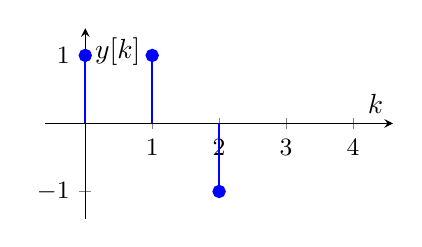
\begin{tikzpicture}
\begin{axis}[
  width=6cm, height=4cm,
  xmin=-0.6, xmax=4.6, ymin=-1.4, ymax=1.4,
  axis lines=middle,
  xlabel={$k$}, ylabel={$y[k]$},
  xtick={0,1,2,3,4}, ytick={-1,1},
  tick label style={font=\small},
]
\addplot+[ycomb, blue, thick, mark=*, mark options={blue}] coordinates {
  (0,1) (1,1) (2,-1)
};
\end{axis}
\end{tikzpicture}
\end{center}

% ---- a) --------------------------------------------------------
\subsubsection*{a) Empirischer Mittelwert von $x[k]$}

\begin{beispiel}[Empirischer Mittelwert des Signals]

\textbf{Gegeben:} $N = 15$ Amplitudenwerte $x[k]$.

\textbf{Gesucht:} $\hat{\bar{x}}$.

\textbf{Formel} (Abschnitt~\ref{sec:lagemasse}):

$$
\hat{\bar{x}} = \frac{1}{N} \sum_{k=0}^{N-1} x[k]
$$

\textbf{Rechnung:}

$$
\sum_{k=0}^{14} x[k]
= -\tfrac12 + 1 + 1 + \tfrac12 - 1 + 1 - \tfrac32 + \tfrac32 + 1 = 3
$$

$$
\hat{\bar{x}} = \frac{3}{15} = \frac{1}{5}
$$

\textbf{Lösung:}

$$
\boxed{\;\hat{\bar{x}} = \frac{1}{5} = 0{,}2\;}
$$

\end{beispiel}

% ---- b) --------------------------------------------------------
\subsubsection*{b) Empirische Varianz von $x[k]$}

\begin{beispiel}[Empirische Varianz des Signals]

\textbf{Gegeben:} $N = 15$, $\hat{\bar{x}} = \tfrac15$.

\textbf{Gesucht:} $\hat{\sigma}^2$.

\textbf{Formel} (Abschnitt~\ref{sec:streumasse}):

$$
\hat{\sigma}^2 = \frac{1}{N-1}\left( \sum_{k=0}^{N-1} x[k]^2 - N\,\hat{\bar{x}}^{\,2} \right)
$$

\textbf{Rechnung:}

$$
\sum_{k=0}^{14} x[k]^2
= \tfrac14 + 1 + 1 + \tfrac14 + 1 + 1 + \tfrac94 + \tfrac94 + 1 = 10
$$

$$
\hat{\sigma}^2 = \frac{1}{14}\left( 10 - 15\cdot\left(\tfrac15\right)^2 \right)
= \frac{1}{14}\left( 10 - \tfrac{3}{5} \right)
= \frac{1}{14}\cdot \frac{47}{5}
= \frac{47}{70}
$$

\textbf{Lösung:}

$$
\boxed{\;\hat{\sigma}^2 = \frac{47}{70} \approx 0{,}671\;}
$$

\end{beispiel}

% ---- c) --------------------------------------------------------
\subsubsection*{c) Median von $x[k]$}

\begin{beispiel}[Median des Signals]

\textbf{Gegeben:} $N = 15$ Amplitudenwerte $x[k]$.

\textbf{Gesucht:} $\tilde{x}$.

\textbf{Formel} (Abschnitt~\ref{sec:lagemasse}): Bei ungeradem $N$ ist der Median
der $\tfrac{N+1}{2} = 8$-te Wert der sortierten Folge.

\textbf{Rechnung:} Sortieren der $15$ Werte:

$$
-\tfrac32,\, -1,\, -\tfrac12,\; 0,\,0,\,0,\,0,\;
\underbrace{0}_{8.\ \text{Wert}},\, 0,\; \tfrac12,\; 1,\,1,\,1,\,1,\; \tfrac32
$$

(Es gibt sechs Nullen an den Positionen $k = 0,3,9,11,12,14$.) Der $8.$ Wert ist
$0$.

\textbf{Lösung:}

$$
\boxed{\;\tilde{x} = 0\;}
$$

\end{beispiel}

% ---- d) --------------------------------------------------------
\subsubsection*{d) Empirische Kreuzkorrelation und Detektion der Codefolge}

\begin{beispiel}[Kreuzkorrelation zur Detektion der Codefolge]

\textbf{Gegeben:} Signal $x[k]$ ($k = 0, \ldots, 14$) und Codefolge
$y[k] = [\,1,1,-1\,]$.

\textbf{Gesucht:} Die empirische Kreuzkorrelation $\hat{\varphi}_{xy}[\varkappa]$
und daraus die Stelle $k$, an der die Codefolge $[\,1,1,-1\,]$ in $x[k]$ beginnt.

\textbf{Formel} (empirische Kreuzkorrelation, Abschnitt~\ref{sec:empirische-korrelation}):

$$
\hat{\varphi}_{xy}[\varkappa] = \sum_{k} x[k]\, y[k + \varkappa]
$$

\textbf{Rechnung:} Da $y[n]$ nur für $n \in \{0,1,2\}$ von null verschieden ist
($y[0]=y[1]=1$, $y[2]=-1$), tragen in der Summe nur die Indizes $k$ mit
$k+\varkappa \in \{0,1,2\}$ bei. Mit $k = -\varkappa,\, 1-\varkappa,\, 2-\varkappa$ folgt

$$
\hat{\varphi}_{xy}[\varkappa]
= x[-\varkappa]\cdot 1 + x[1-\varkappa]\cdot 1 + x[2-\varkappa]\cdot(-1)
= x[-\varkappa] + x[1-\varkappa] - x[2-\varkappa].
$$

Ein positiver Beitrag entsteht also dort, wo $x$ dem Muster $[\,1,1,-1\,]$ ähnelt.
Auswertung für $\varkappa = 0, -1, \ldots, -12$:

\begin{center}
\renewcommand{\arraystretch}{1.3}
\begin{tabular}{c|c|c}
$\varkappa$ & $x[-\varkappa] + x[1-\varkappa] - x[2-\varkappa]$ & $\hat{\varphi}_{xy}[\varkappa]$ \\
\hline
$0$    & $x[0]+x[1]-x[2] = 0-\tfrac12-1$        & $-\tfrac32$ \\
$-1$   & $x[1]+x[2]-x[3] = -\tfrac12+1-0$       & $\tfrac12$ \\
$-2$   & $x[2]+x[3]-x[4] = 1+0-1$               & $0$ \\
$-3$   & $x[3]+x[4]-x[5] = 0+1-\tfrac12$        & $\tfrac12$ \\
$-4$   & $x[4]+x[5]-x[6] = 1+\tfrac12-(-1)$     & $\mathbf{\tfrac52}$ \\
$-5$   & $x[5]+x[6]-x[7] = \tfrac12-1-1$        & $-\tfrac32$ \\
$-6$   & $x[6]+x[7]-x[8] = -1+1-(-\tfrac32)$    & $\tfrac32$ \\
$-7$   & $x[7]+x[8]-x[9] = 1-\tfrac32-0$        & $-\tfrac12$ \\
$-8$   & $x[8]+x[9]-x[10] = -\tfrac32+0-\tfrac32$ & $-3$ \\
$-9$   & $x[9]+x[10]-x[11] = 0+\tfrac32-0$      & $\tfrac32$ \\
$-10$  & $x[10]+x[11]-x[12] = \tfrac32+0-0$     & $\tfrac32$ \\
$-11$  & $x[11]+x[12]-x[13] = 0+0-1$            & $-1$ \\
$-12$  & $x[12]+x[13]-x[14] = 0+1-0$            & $1$ \\
\end{tabular}
\end{center}

\begin{center}
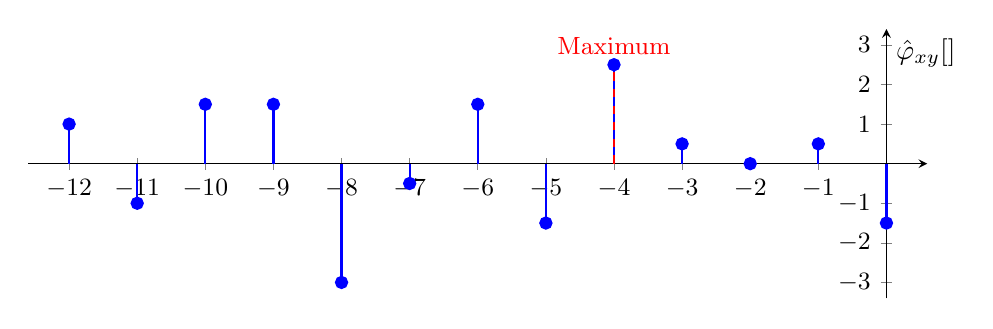
\begin{tikzpicture}
\begin{axis}[
  width=13cm, height=5cm,
  xmin=-12.6, xmax=0.6, ymin=-3.4, ymax=3.4,
  axis lines=middle,
  xlabel={$\varkappa$}, ylabel={$\hat{\varphi}_{xy}[\varkappa]$},
  xtick={-12,-11,-10,-9,-8,-7,-6,-5,-4,-3,-2,-1,0},
  ytick={-3,-2,-1,1,2,3},
  tick label style={font=\small},
]
\addplot+[ycomb, blue, thick, mark=*, mark options={blue}] coordinates {
  (0,-1.5) (-1,0.5) (-2,0) (-3,0.5) (-4,2.5) (-5,-1.5) (-6,1.5)
  (-7,-0.5) (-8,-3) (-9,1.5) (-10,1.5) (-11,-1) (-12,1)
};
\addplot[red, dashed, thick] coordinates {(-4,0) (-4,2.5)};
\node[red, anchor=south, font=\small] at (axis cs:-4,2.5) {Maximum};
\end{axis}
\end{tikzpicture}
\end{center}

Das ausgeprägte Maximum liegt bei $\varkappa = -4$ mit
$\hat{\varphi}_{xy}[-4] = \tfrac52$. Für $\varkappa = -4$ überlappt die
Codefolge $y$ gerade die Werte $x[4], x[5], x[6]$; die Codefolge beginnt also bei
$k = 4$. Tatsächlich passt das Muster $[\,1,1,-1\,]$ dort am besten:
$x[4] = 1$, $x[5] = \tfrac12$, $x[6] = -1$.

\textbf{Lösung:}

$$
\boxed{\;\max_{\varkappa} \hat{\varphi}_{xy}[\varkappa]
= \hat{\varphi}_{xy}[-4] = \frac{5}{2}
\quad\Longrightarrow\quad
\text{Codefolge beginnt bei } k = 4.\;}
$$

Dies ist das Prinzip eines Korrelationsdetektors (vgl.\
Abschnitt~\ref{sec:signalentdeckung-rauschen}): Die bekannte Codefolge wird über
das Signal geschoben, und das Maximum der Kreuzkorrelation markiert die Stelle
der besten Übereinstimmung.

\end{beispiel}
